\documentclass[cn,table]{elegantbook}

\usepackage{tikz}
\usepackage{graphicx}
\usepackage{subcaption}
\usepackage[ruled,linesnumbered,vlined]{algorithm2e}
\usepackage{hyperref}
\usepackage{listings}
\usepackage{interval}
\usepackage{xcolor}
\usepackage{ulem}
\usepackage{wrapfig}

\intervalconfig{%
	soft open fences,
}

\def\figureautorefname{图}
\def\sectionautorefname{小节}

\SetAlgorithmName{算法}{算法}{算法索引}

\renewcommand*{\lstlistingname}{代码}

\title{何老师算法课笔记}
\subtitle{Always be patient, sharp and diligent.}
\author{计卓1801全体}
\institute{华中科技大学}
\date{\zhtoday}
\version{1.8.0}
\logo{logo.png}
\cover{cover.png}

\begin{document}
\maketitle
\tableofcontents
\pagenumbering{arabic}

% add your code here
% \input{src/example.tex}
\input{src/Ln1-AsymptoticOrderGrowth.tex}
\input{src/Tiling-Problem.tex}
\input{src/stable-matching.tex}
\chapter{图算法之最小生成树}

\begin{introduction}
	\item 问题概述
	\item Prim算法
	\item Kruskal算法
\end{introduction}

\section{概述}
给定一张边带权的无向图G=(V, E),其中V表示图中点的集合,E表示图中边的集合,n=|V|,m=|E|。
由V中的全部n个顶点和E中n-1条边构成的无向连通子图被称为G的一棵生成树,其中边的权值之和最小的生成树被称为无向图G的最小生成树。

最小生成树最为经典的两个算法分别是Prim算法和Kruskal算法。本节将首先讨论这两个算法的执行过程。

\section{基本概念}
在深入探讨之前,还需明白一些定义:

\begin{definition}{path}{path}
	A path is a sequence of edges which connects a sequence of nodes.
\end{definition}

\begin{definition}{cycle}{cycle}
	A cycle is a path with no repeated nodes or edges other than the
starting and ending nodes.
\end{definition}

可以借助\autoref{fig:path-cycle}理解path以及cycle的概念。

\begin{figure}[hbt]
	\centering
	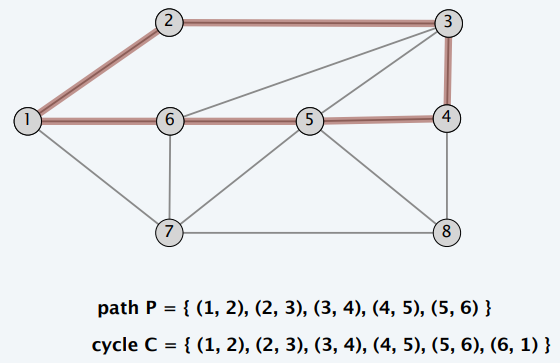
\includegraphics[scale=0.5]{image/pathcycle.png}
	\caption{具体例子说明path和cycle}\label{fig:path-cycle}
\end{figure}

\begin{definition}{cut}{MSTcut}
	A cut is a partition of the nodes into two nonempty subsets S and V / S.
\end{definition}

\begin{definition}{cutset}{MSTcutset}
	The cutset of a cut S is the set of edges with exactly one endpoint in S.
\end{definition}

可以借助\autoref{fig:cut-cutset}理解cut以及cutset的概念。

\begin{figure}[hbt]
	\centering
	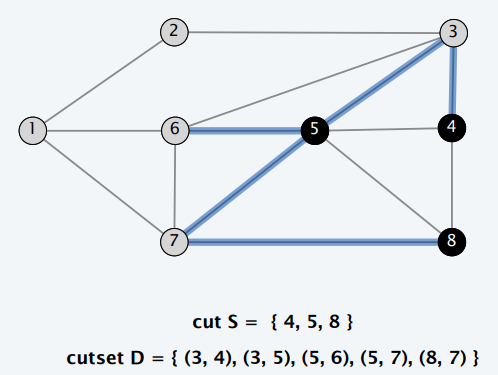
\includegraphics[scale=0.5]{image/cutcutset.png}
	\caption{具体例子说明cut与cutset}\label{fig:cut-cutset}
\end{figure}

\begin{theorem}{}{cycle-cutset-theorem}
	A cycle and a cutset intersect in an even number of edges.
\end{theorem}

可以借助\autoref{fig:cycle-cutset}理解\autoref{cycle-cutset-theorem}。

\begin{figure}[hbt]
	\centering
	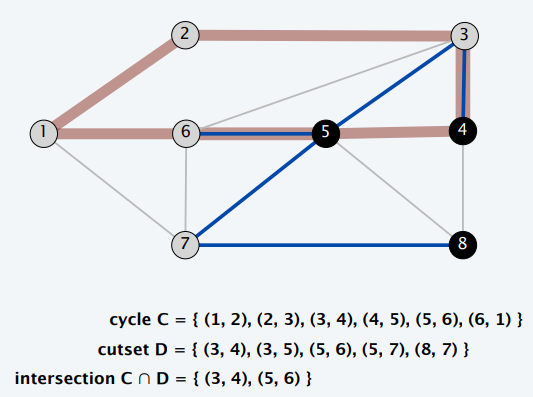
\includegraphics[scale=0.5]{image/cyclecutset.png}
	\caption{cycle、cutset的性质}\label{fig:cycle-cutset}
\end{figure}

\begin{definition}{生成树}{ST}
Let H = (V, T) be a subgraph of an undirected graph G = (V, E).
H is a spanning tree of G if H is both acyclic and connected.
\end{definition}

一个生成树的例子如\autoref{fig:exampleofST}所示。

\begin{figure}[hbt]
	\centering
	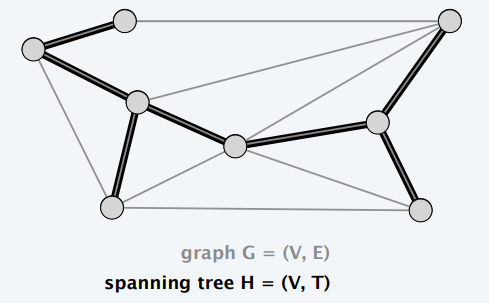
\includegraphics[scale=0.5]{image/exampleofST.png}
	\caption{生成树的例子}\label{fig:exampleofST}
\end{figure}

\begin{theorem}{}{ST-theorem}
	如果H = (V, T)是一个无向图G = (V, E)的子图,那么,以下各条件等价:
	\begin{enumerate}
		\item H是G的一棵生成树
		\item H是无环且连通的
		\item H是连通的并且有 V – 1条边
		\item H是无环的并且有 V – 1条边
		\item 任意拿掉H的一条边,就不再使其连通
		\item 任意增加一条边,则H就会构成环
	\end{enumerate}

\end{theorem}

\begin{definition}{最小生成树}{MST}
	Given a connected, undirected graph G = (V, E) with edge costs $c_e$,
a minimum spanning tree (V, T) is a spanning tree of G such that the sum
of the edge costs in T is minimized.
\end{definition}

一个生成树的例子如\autoref{fig:exampleofMST}所示。

\begin{figure}[hbt]
	\centering
	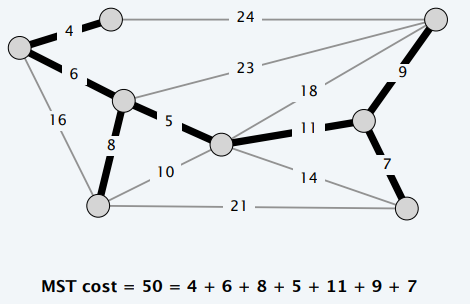
\includegraphics[scale=0.5]{image/exampleofMST.png}
	\caption{生成树的例子}\label{fig:exampleofMST}
\end{figure}

\begin{theorem}{Cayley’s theorem}{Cayley-theorem}
	The complete graph on n nodes has $n^(n–2)$ spanning trees
\end{theorem}

最小生成树是一个基础却有着十分广泛的应用的问题,之后的\autoref{sec:prim}和\autoref{sec:kruskal}
将分别介绍求解最小生成树的Prim算法和Kruskal算法。

\section{Prim算法}\label{sec:prim}
\subsection{算法描述与演示}
\begin{algorithm}
	\DontPrintSemicolon
	\KwIn{Graph G}
	\KwResult{MST of Graph G}
	\Begin{
		$S \leftarrow \{ s \} $ for any node s,$T \leftarrow \emptyset$;\\
		\For{$|T| < n-1$}{
			Add to T a min-weight edge with exactly one endpoint in S;\\
			Add the other endpoint to S;\\
		}
		Return T ;\\
	}
	\caption{Prim}\label{alg:Prim}
\end{algorithm}

算法执行流程如\autoref{fig:Prim}所示。

\begin{figure}[hbt]
	\centering
	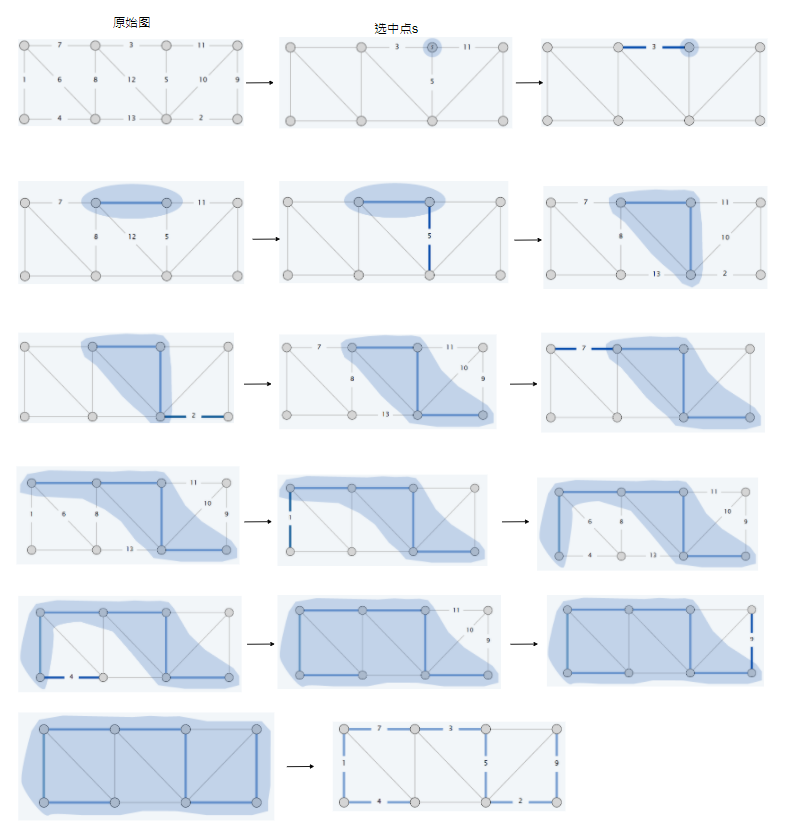
\includegraphics[scale=0.5]{image/prim.png}
	\caption{Prim算法的执行流程}\label{fig:Prim}
\end{figure}

\subsection{算法正确性证明}
\noindent记图G是一个连通图,Y是对p使用prim算法得到的一棵生成树,$Y_1$是p的一棵最小生成树
\begin{enumerate}
	\item 若Y=$Y_1$,显然prim算法是正确的
	\item 若Y≠$Y_1$,可进行如下推导:

	a)Y中有$n( n \geq 1 )$条边不存在于$Y_1$中,在构建Y的过程中,第一次遇到这样的一条边时(以e表示),
	则e的一个端点u落在V内(V是之前的prim运算得到的一个子顶点集),另一个端点v落在V外
	
	b)$Y_1$是连通的,故$Y_1$中存在u到v的一条的路径,此路径上必然存在一条边f,它的一个端点落在V内,另一个端点落在V外
	
	c)把e加入$Y_1$,去掉f,$Y_1$仍然连通,根据prim算法,权值$W(f) \geq W(e)$,否则e不会被选入V,
	如果$W(f)>W(e)$,新构建的树的权值和会比$Y_1$小,而$Y_1$是最小生成树,因此$W(f)>W(e)$不成立,得$W(f)=W(e)$
	
	d)对每一条类似e的边,重复过程c),最终Y和重新构建的的$Y_1$拥有的边完全一致,
	新构建的$Y_1$也是最小生成树,因此Y也是最小生成树,证明prim算法正确
\end{enumerate}

\subsection{算法复杂度}
普通堆优化的 Prim 算法复杂度为 $O(mlogn)$,而斐波那契堆优化的 Prim 算法
能达到 $O(m+nlogn)$

\section{Kruskal算法}\label{sec:kruskal}
\subsection{算法描述与演示}
\begin{algorithm}
	\DontPrintSemicolon
	\KwIn{Graph G}
	\KwResult{MST of Graph G}
	\Begin{
		$T \leftarrow \emptyset$;\\
		$S \leftarrow$sort edges by weight;\\
		\While{$e \in S$}{
			\If{$T \cup \{ e \}$ no cycle}{
				$T = T \cup \{ e \};$
			}
			\If{$|T| < n-1$}{
				Return T ;\\
			}
		}
	}
	\caption{kruskal}\label{alg:kruskal}
\end{algorithm}

算法执行流程如\autoref{fig:kruskal}所示。

\begin{figure}[hbt]
	\centering
	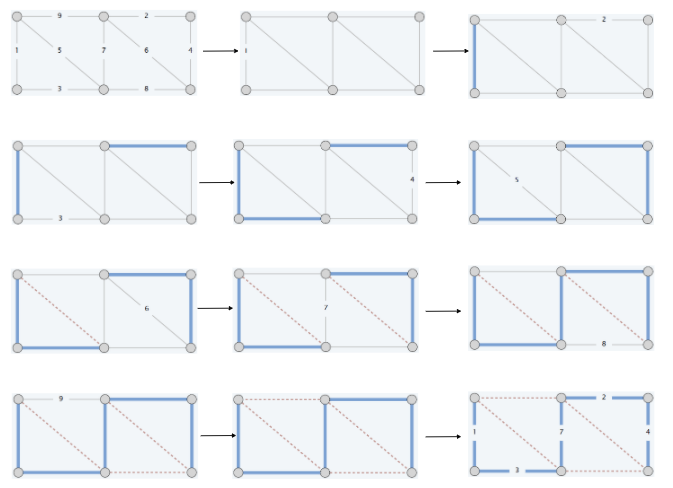
\includegraphics[scale=0.5]{image/kruskal.png}
	\caption{Kruskal算法的执行流程}\label{fig:kruskal}
\end{figure}

\subsection{算法正确性证明}
Kruskal算法每次会向T添加一条最小权重的边,并且不能形成环.
对于一棵树而言, 如果有K个节点, 则必然有K-1条边
我们要证明的问题其实是连续添加的边E(l) l=0,1,2...K-1 是一颗最小生成树MST的子集.

对于基本情况, 如果I = 0, 此时为空集,满足条件;

现在我们假设对 $0 \leq m < K-1$, E(m) 已经满足条件,是$T_1$的子集. 我们来看 E(m+1)的情况,
有E(m+1) = E(m) + {e}, e为算法当前新增的最小权重边.此时分两种情况:

\begin{enumerate}
	\item 如果{e}是$T_1$的子集,那么问题解决;
	\item 如果{e}不是$T_1$的子集, 那么我们要证明 E(m+1) 属于一颗其他的MST子集:

	因为{e}不是$T_1$的边, 所以 $T_1$ + {e} 必然有环C(性质1), 同时 E(m) 属于 $T_1$ ,
	那么在环C上必然有一个{e'} 不属于E(m) (因为如果属于E(m)的化, 那么算法当前选择的{e}会导致一个环, 与性质1违背).
	
	现在我们定义$T_2$ = $T_1$ + {e} - {e'}, 又因为E(m+1) = E(m) + {e} 所以 E(m+1) 属于$T_2$的子集.$T_2$是一颗MST.
	
	因为{e} 和 {e'} 都不属于 E(m), 算法当前选择的是{e} 说明 $weight({e'}) \geq weight({e})$.
	所以我们看$weight(T_2) = weight(T_1) + weight({e}) - weight({e'}) \leq weight(T_1)$ .
	
	这意味着$T_1$是$T_2$的权重upper-bound, 但由于$T_1$已经是MST, 所以必然的$T_2$也是MST. 至此得证.	
\end{enumerate}

\subsection{算法复杂度分析及优化}
\begin{theorem}{}{Kruskal-theorem}
	Kruskal’s algorithm can be implemented to run in $O(m log m)$ time.
\end{theorem}

\begin{enumerate}
	\item Sort edges by cost:$O(m log m)$.
	\item Use union–find data structure to dynamically maintain connected components:$O(m \alpha (n))$.
\end{enumerate}

\begin{remark}
	$\alpha (n)$是反阿克曼函数,阿克曼函数 $A(m,n)$ 增长极快,其反函数几乎是常数。
\end{remark}

下面将简要介绍并查集(union–find data structure)有关内容。
\subsection{并查集}
在计算机科学中,并查集是一种树型的数据结构,用于处理一些不交集(Disjoint Sets)的合并及查询问题。
有一个联合-查找算法(union-find algorithm)定义了两个用于此数据结构的操作:

Find:确定元素属于哪一个子集。它可以被用来确定两个元素是否属于同一子集。

Union:将两个子集合并成同一个集合。

在并查集森林中,每个集合的代表即是集合的根节点。“查找”根据其父节点的引用向根行进直到到底树根。
“联合”将两棵树合并到一起,这通过将一棵树的根连接到另一棵树的根。实现这样操作的一种方法是

\begin{lstlisting}
function MakeSet(x)
     x.parent := x

function Find(x)
     if x.parent == x
        return x
     else
        return Find(x.parent)

function Union(x, y)
     xRoot := Find(x)
     yRoot := Find(y)
     xRoot.parent := yRoot
\end{lstlisting}

这是并查集森林的最基础的表示方法,这个方法不会比链表法好,这是因为创建的树可能会严重不平衡;然而,可以用两种办法优化。

第一种方法,称为“按秩合并”,即总是将更小的树连接至更大的树上。因为影响运行时间的是树的深度,
更小的树添加到更深的树的根上将不会增加秩除非它们的秩相同。在这个算法中,术语“秩”替代了“深度”,因为同时应用了路径压缩时秩将不会与高度相同。

第二个优化,称为“路径压缩”,是一种在执行“查找”时扁平化树结构的方法。关键在于在路径上的每个节点都可以直接连接到根上;
他们都有同样的表示方法。为了达到这样的效果,Find递归地经过树,改变每一个节点的引用到根节点。得到的树将更加扁平。

\chapter{最小生成树其他算法}

\begin{introduction}
	\item red/blue算法
	\item Boruvka算法
\end{introduction}

本章将介绍求解最小生成树的red/blue算法和Boruvka算法。

\section{red/blue算法}

\subsection{基本概念}
下面给出red/blue算法有关内容的定义
\begin{definition}{割(cut)}{cut}
	S$\in$V,S$\neq \emptyset$,点集V被划分成互补的子集S和V/S。
\end{definition}

\begin{definition}{割边集(cutset)}{cutset}
    对于图G的顶点集V的割X、Y,图G的边集E中连接两集合X、Y的所有边的集合叫做这个割的割边集(cutset)。
\end{definition}

\begin{definition}{Red Rule}{Red Rule}
    找到图G中不含红色边的环C,从C中未被染色的边中选出边权最大的边将其染成红色。
\end{definition}

\begin{definition}{Blue Rule}{Blue Rule}
    找到图G中不含蓝色边的割边集D,从D中未被染色的边中选出边权最小的边将其染成蓝色。
\end{definition}

\subsection{算法运行步骤}
\begin{enumerate}
	\item 初始化:对于给定的图G,将所有边标记为未染色。
	\item 在图G中同时运行Red Rule和Blue Rule (可并行运行),直到所有边均被染色为止。
	\item 图G中所有的蓝色边即为图G的最小生成树。
\end{enumerate}

算法具体执行过程如\autoref{fig:redblue}
\begin{figure}[hbt]
	\centering
	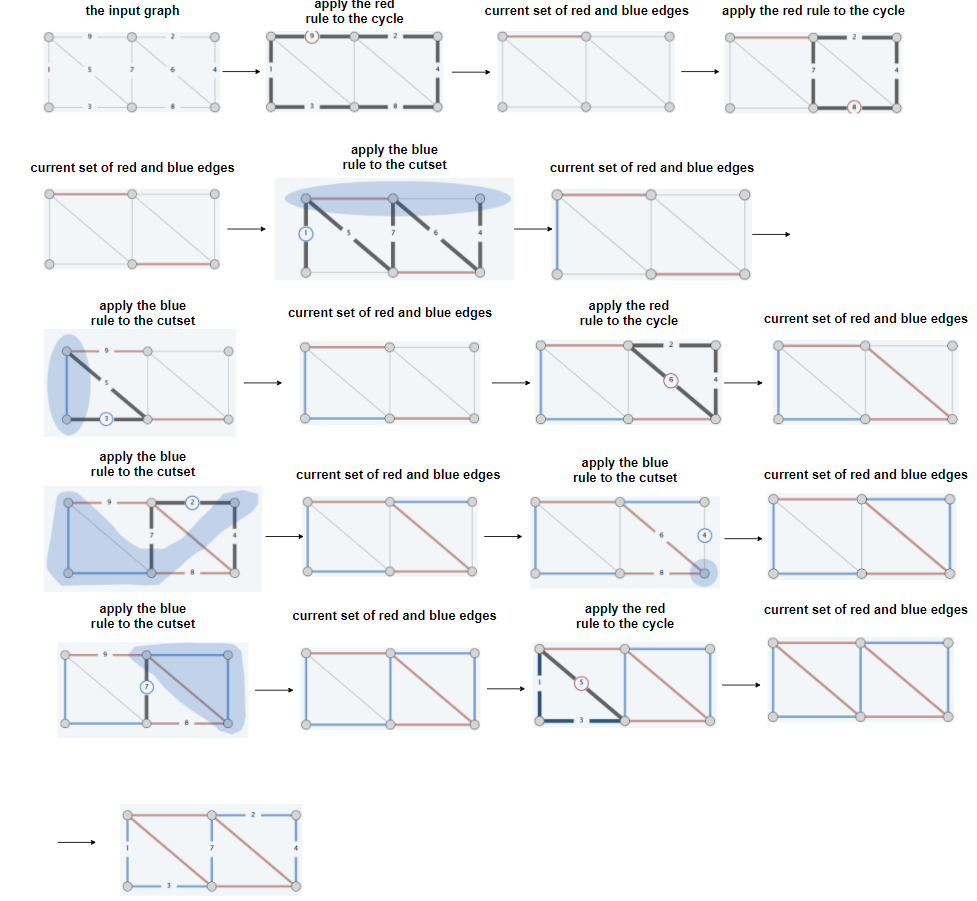
\includegraphics[scale=0.4]{image/redblue.png}
  \caption{red/blue算法执行过程图解}\label{fig:redblue}
\end{figure}

\subsection{算法正确性证明}\label{sec:redblue-proof}
\begin{enumerate}
	\item 最优性:Blue Rule染色所得边为最小边

对于图G中的一个割边集D及D中边权最小的边minEdge,如果在Blue Rule运行过程中被染色的是割边集D的其他边biggerEdge,
则可以在最后得到的MST中将biggerEdge从中删除然后将minEdge加入到MST中,可以得到更小的最小生成树。产生矛盾。所以Blue Rule染色所得边为最小边。
\item 合法性:算法所得所有蓝边为无环连通图

由于Blue Rule可知每次选边都不会成环。下证所得为连通图,假设最后所得所有蓝边构成的图不连通或仍然有点未被蓝边连接。

对于第一种情况,则任选某一蓝边的一个顶点并从该顶点开始的所有能通过蓝边的顶点记为集合X,
S与V/S构成图G的一个割,由Red Rule中所选环C不含红色边可知其割边集不可能全部被染成红色,则说明一定有未染色的边,再应用一次Blue Rule即可增大S的点的个数,
重复上述过程直到S=E;对于第二种情况,由于孤立点必不可能在某个环中,所以连接该点的边一定不会被Red Rule染成红色,所以此时应用一次Blue Rule即可使得该点被蓝边连接。综上,算法所得所有蓝边为连通图
\end{enumerate}

\section{Boruvka算法}
\subsection{算法运行步骤}
\begin{enumerate}
	\item 初始化:对于给定的图G,将所有边标记为未染色;将每个顶点作为一个连通块。
	\item 对于所有蓝边连成的连通块应用Blue Rule并将所有Blue Rule选中的边染成蓝色,直到只有一个连通块。
	\item 最后得到的蓝边连成的连通块即为图G的最小生成树。
\end{enumerate}

算法具体执行过程如\autoref{fig:boruvka}
\begin{figure}[h]
	\centering
	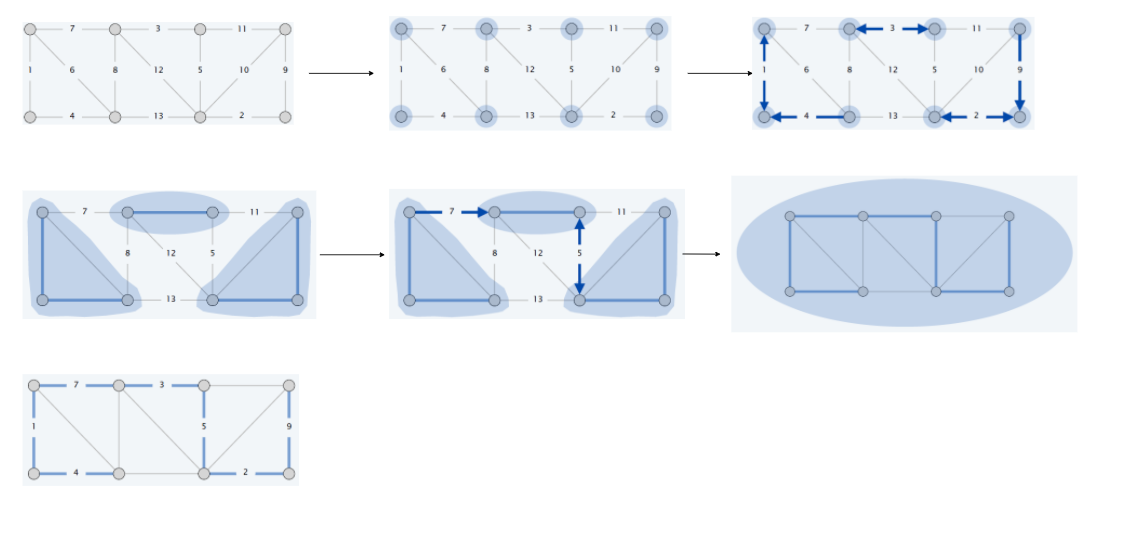
\includegraphics[scale=0.4]{image/boruvka.png}
  \caption{boruvka算法执行过程图解}\label{fig:boruvka}
\end{figure}

算法复杂度分析:每次应用Blue Rule后连通块数量至少减半,每次都要遍历所有边,所以算法串行时间复杂度为O(E$\log V$),并行时间复杂度为O(E)。

\subsection{算法正确性证明}
\begin{enumerate}
	\item 最优性:根据~\ref{sec:redblue-proof}中的证明:Blue Rule染色所得边为最小边。
	\item 合法性:一定不会构成环。如果存在环说明一个点的最小连边有两个,与Blue Rule矛盾。
\end{enumerate}

\input{src/Ln9-NearestPoints.tex}
\input{src/Ln11-LargeIntegerMultiplication.tex}
\input{src/dynamic-programming-1.tex}
\input{src/LN18-DP-ZeroOneKnapsack.tex}
\chapter{动态规划之上下文无关文法}\label{header-n1150}

\begin{introduction}
	\item 综述
	\item 上下文无关文法及其派生树
	\item CYK算法
\end{introduction}

\section{综述}\label{header-n1151}

\begin{itemize}
\item
  上下文无关语言是一种形式语言(形式语言指在某个字母表上一些有限长字串的集合)。生成这种语言的文法叫做上下文无关文法,常用于计算机中语法分析器(Parsers)的构造。
\item
  关于这个文法的具体使用在编译原理(以及计算理论)课程中会有详细的介绍,在这里我们只简要介绍其基本概念,着重介绍一个和上下文无关文法有关的动态规划算法------CYK算法(The
  CYK Parsing Algorithm)
\end{itemize}

\section{上下文无关文法及其派生树}\label{header-n1157}

\subsection{上下文无关文法}\label{header-n1158}

\begin{itemize}
\item
  下面先举一个上下文无关文法的例子(S为文法的source):
\end{itemize}

\(S\rightarrow aBb\) \quad
\(B\rightarrow aBb|\epsilon\)

\begin{itemize}
\item
  根据这个文法,如果我们想生成串aaabbb,可以进行如下推导:
\end{itemize}

\(S\Rightarrow aBb \Rightarrow aaBbb \Rightarrow aaaBbbb \Rightarrow aaa\epsilon bbb \Rightarrow aaabbb\)

\begin{itemize}
\item
  形式化地,我们将上下文无关文法定义成如下四元组形式:

  \begin{itemize}
  \item
    \(G=(V,T,S,P)\),其中\(G\)代表文法,\(V\)代表文法中的变量,\(T\)代表文法最终到达的常量,\(S\)代表文法的起始变量(source),\(P\)代表由变量和常量生成的文法。
  \item
    具体的,在上述文法中:

    \begin{itemize}
    \item
      \(V=\{S,B\}\)
    \item
      \(T=\{a,b\}\)
    \item
      \(S=\{S\}\)
    \item
      \(P=\{S\rightarrow aBb , B\rightarrow aBb|\epsilon\}\)
    \end{itemize}
  \end{itemize}
\item
  上述上下文无关文法对应语言:\(L=\{a^nb^n|n为大于或等于1的整数\}\)
\end{itemize}

\subsection{派生树}\label{header-n1186}

\begin{itemize}
\item
  上下文无关文法的派生数指的是把由上下文无关文法生成上下文无关语言的过程用树的形式表示出来,比如19.1.1中的文法可以表示成以下派生树:
\end{itemize}

\begin{itemize}
\item
  可以总结出,派生树的画法是,以S(soruce)节点作为根节点,父节点对应文法的左边,子节点对应文法的右边,建立派生树得到最后的串。最后,从左到右叶子结点的值就是最后生成的串。
\end{itemize}

\section{CYK算法}\label{header-n1194}

\begin{itemize}
\item
  CYK算法是一种基于动态规划思想的算法,要解决的问题是:给定串w,测试这个串是否能够用起始变量S生成。其算法的复杂度为\(O(n^3)\)
\item
  CYK算法是由发现相同思想的三个人J. Cocke、 D. Younger和T.
  Kasami的名字来命名的。
\item
  CYK算法不适用于在所有的context free
  language上直接使用,先要转换成乔姆斯基范式(Chomsky Normal
  Form)才能实现。
\end{itemize}

\subsection{CNF(乔姆斯基范式)}\label{header-n1201}

\begin{itemize}
\item
  文法只包含以下两种形式:
\end{itemize}

\(A\rightarrow BC\) \quad
\(A\rightarrow a\)

\begin{itemize}
\item
  概括来说,即只能由变量生成两个变量或者生成一个最终常量
\item
  转换方法如下:

  \begin{itemize}
  \item
    将常量全部添加\(T_a\rightarrow a\)形式,替换其他生成式中所有的常量为变量
  \item
    将文法右侧所有的多变量变成二变量,即把\(A\rightarrow A_0A_1A_2\)替换成\(A\rightarrow A_0B,B\rightarrow A_1A_2\)形式(多变量同理)
  \end{itemize}
\item
  一个转换的例子如下:

  \begin{itemize}
  \item
    原文法:\(S\rightarrow ABa,A\rightarrow aab,B\rightarrow Ac\)
  \item
    转换后文法:\(S\rightarrow AV_1,V_1\rightarrow BT_a,A\rightarrow T_aV_2,V_2\rightarrow T_aT_b,B\rightarrow AT_c,T_a\rightarrow a,T_b\rightarrow b,T_c\rightarrow c\)
  \end{itemize}
\end{itemize}

\subsection{CYK算法的基本内容}\label{header-n1224}

\begin{itemize}
\item
  问题的形式化定义:对于一个上下文无关文法G和一个给定的串\(w=a_1a_2...a_n\),求解是否存在一种推导(或一棵对应的派生树),使得G能够从S(source)生成对应的字串。
\item
  动态规划的做法是,构造一个动态规划的表(这里以n=5为例子),如下图所示。

  \begin{itemize}
  \item
    水平轴对应串\(w=a_1a_2...a_5\)
  \item
    表中\(x_{ij}\)对应着能够满足生成\(A\Rightarrow a_ia_{i+1}...a_j\)的变元A的集合。
  \item
    最后,如果source点S属于集合\(x_{1n}\),证明这个串可以由S生成,否则则不行。
  \end{itemize}
\end{itemize}

\subsection{算法一个具体例子上的执行过程}\label{header-n1238}

\begin{itemize}
\item
  这一小节我们将用一个例子模拟CYK算法的执行过程,下一节将在此基础上归纳写出CYK算法的关键,也就是动态规划算法的转移方程
\item
  考虑以下这个上下文无关文法,我们用其派生树生成了一个长度为7的串,如下图:
\end{itemize}

\begin{itemize}
\item
  对于串\(aaaabab\),我们构造上述所说的动态规划表如下:
\end{itemize}

\begin{itemize}
\item
  对于上述动态规划表给出说明:

  \begin{itemize}
  \item
    首先求解第一行(\(x_{ii}\))有,其对应的集合就是生成字符串中每一个字符(常量)的源头的集合。例如常量a可以由变量A和C生成,所以其集合就是\{A\textbar C\},常量b可以由变量B生成,所以其对应的集合就是\{B\}。
  \item
    从第二行开始,其结果完全依赖于第一行,例如\(x_{12}\)对应着字符串aa,我们将串aa分成两份,有且只能被分割为第一个a和第二个a这一种情况,那么要求解\(x_{12}\)的值,需要做下面两步:

    \begin{itemize}
    \item
      求出\(x_{11}\)和\(x_{22}\)的笛卡尔积。算出结果为\{AA\textbar AC\textbar CA\textbar CC\}。
    \item
      寻找该笛卡尔积中的每一个元素对应的源头。例如AA、AC、CA都没有对应的,则都为空集,AC对应的源头为\{B\}。最后的结果将这四个集合求并集,得到\(x_{12}\)的值为\{B\}
    \end{itemize}
  \item
    第二行其余项的算法同计算\(x_{12}\)类似。
  \item
    第三行开始,每一个串都有多个划分,比如求解\(x_{13}\),对应的串为aaa,我们就有两种划分,aa和a、a和aa,那么求解\(x_{13}\)只用遵循以下步骤即可:

    \begin{itemize}
    \item
      分别用第二行的策略求出\(x_{12}\)和\(x_{33}\)的笛卡尔积,再寻找其源头,得到第一个集合;求出\(x_{11}\)和\(x_{33}\)的笛卡尔积再寻找其源头,得到第二个集合。
    \item
      将上述两个集合求并集得到\(x_{13}\)的结果
    \end{itemize}
  \item
    第三行其余项的算法同理。
  \item
    从第四行开始往上走,处理策略与第三行类似,只不过是对于要求解串的划分情况更多了而已。例如\(x_{15}\)对应aaaab,这个串有4种划分情况,将每种情况的笛卡尔积求源头,得到四个集合,对这四个集合求并集即得到\(x_{15}\)的结果。
  \end{itemize}
\item
  下面我们将给出求解\(x_{ij}\)一般化的公式
\end{itemize}

\subsection{19.3.4 状态转移方程以及算法伪代码}\label{header-n1277}

\begin{itemize}
\item
  由上述举例我们已经了解到了具体的求解\(x_{ij}\)(从生成串的索引i到索引j对应的源头)的方法,这里归纳给出一般化公式即可:

  \begin{itemize}
  \item
    首先给出一个函数souce(s),其中s为一个集合或者一个字符(i=1时候),函数功能是求出s对应的源头的集合,例如\(source(a)=\{A|C\}\),\(source(\{AA|AC|CA|CC\})={B}\)。
  \item
    基于求源头函数给出状态转移方程(假设原始串被存在数组a{[}N{]}中,串长为n,下标从1开始):
  \end{itemize}

  \(x_{ij}=\begin{cases}\bigcup_{k=i}^{k=j}source(x_{ik}\times x_{kj})& \text{j>i}\\source(a[i])& \text{j=i}\end{cases}\)

  \begin{itemize}
  \item
    注:上述公式中\(\times\)符号代表笛卡尔积
  \end{itemize}
\item
  给出算法的为代码如下(假设原始串被存在数组a{[}N{]}中,串长为n,下标从1开始):
\end{itemize}

\begin{lstlisting}[language = C++, caption = 算法伪代码]
context_free(a[N])
{
    int dp[N][N] //存表
    from len=1 to n //按照串长从1到n,横向计算每一行
        from i=1 to n-len+1 //计算每一行,索引值从1开始到n-len+1
            j=i+len-1
            dp[i][j]=compute xij //按照状态转移方程计算dp[i][j]
    if(S belongs to dp[1][n]) //如果起始点S在dp[1][n]中,这个串就可生成,否则不能生成
        return true
    else 
        return false
}
\end{lstlisting}

\subsection{算法复杂度分析}\label{header-n1293}

\begin{itemize}
\item
  算法复杂度分析如下:

  \begin{enumerate}
  \def\labelenumi{\arabic{enumi}.}
  \item
    要构建整张动态规划表,需要循环次数\(O(n^2)\)
  \item
    每一次循环中,执行\(compute\)
    \(x_{ij}\),其中我们语法中变量个数为常数个,即\(O(1)\),其笛卡尔积的复杂度为\(O(1)\times O(1)=O(1)\)。而我们要对每一个笛卡尔积作不相容的合并操作(即合并集合中没有相同元素),最多合并n-1次,每个集合中元素数量为常数级,这一步不相容union复杂度为\(O(n)\)
  \item
    综上,总复杂度为\(O(n)\times O(n^2)=O(n^3)\)
  \end{enumerate}
\end{itemize}

\chapter{网络流}

\begin{introduction}
	\item 网络流
	\item 最大流
	\item Ford-Fulkerson算法
	\item 残差图与增广路径
\end{introduction}

\section{网络流}

\subsection{什么是网络流}

	\par 简单地说,网络流是图上的一种映射关系,但也可以理解为一个图生成的一个有向子图,且这个子图受到图本身条件的限制。
		形象地说,就好比一个管道网络和其中流淌的水。下面给出网络流的形式化描述。

\begin{definition}{网络流定义}{network-flow}
	对有向图\(G(V, E)\),
	图中有源点\(s\)和汇点\(t\),且\(s, t \in V,\ s \ne t\),
	\(E\)中边的容量\(C\)是一个映射\(C:E \to N\ or\ R^+\)。
	定义流(flow)是\((G, C)\)上的一个映射\(f:E \to N\ or\ R^+\),满足下列约束:
	
	\begin{enumerate}[(1)]
	\item 容量限制:对\(\forall\ e \in E,\ f(e) \le C(e)\);
	
	\item 流量守恒:对\(\forall\ v \in V / \{s, t\},\ f_{in}(v) = f_{out}(v)\),
	其中
	\begin{equation}\nonumber
	f_{in}(v) = \sum_{(u,v) \in E, u \in V} f(u,v)
	\end{equation}
	\begin{equation}\nonumber
	f_{out}(v) = \sum_{(v,u) \in E, u \in V} f(v,u)
	\end{equation}
	
	特别地,\(s\)的入度、\(t\)的出度为0。
	\end{enumerate}

\end{definition}

	\par 对于一个网络流,我们通常使用流的价值(大小)来进行评价。流的价值描述如下。

\begin{definition}{流的价值}{value-of-a-flow}
	一个网络流\(f\)的价值记为\(|f|\),有
	
	\begin{equation}
	|f| = \sum_{(s,v) \in E, v \in V} f(s,v) = \sum_{(v,t) \in E, v \in V} f(v,t)
	\end{equation}
	
	也就是源点\(s\)的出度、汇点\(t\)的入度。
	
\end{definition}

\subsection{网络流的\(s-t\)割}

	\par 为了辅助分析网络流,引入\(s-t\)割的概念。

\begin{definition}{\(s-t\)割}{s-t-cut}
	一个\(s-t\)割是对点的一种划分,记为\(cut(A, B)\),将图\(G\)的点集\(V\)划分成\(A, B\)两部分,使得
	\(A \cup B = V,\ A \cap B = \varnothing,\ s \in A,\ t \in B\)。
\end{definition}

	\par 注意,这与通常所说的割集有所不同。\(s-t\)割是一种划分方式,而割集是边的集合。
	对一个连通图而言,去掉一个割集中的所有边,将使得这个图不再连通,分为\(A,\ B\)两个连通子图;但若少去掉其中的任何一条,它仍然还是连通的。

\begin{proposition}{\(s-t\)割的性质}{s-t-cut-prop}
	对\(\forall f\), \(\forall cut(A, B)\)有
	\begin{equation}
		f(A,B) \triangleq \sum_{u \in A, v \in B, (u,v) \in E} f(u,v) - \sum_{u \in A, v \in B, (v,u) \in E} f(v,u) = |f|
	\end{equation}
\end{proposition}

\begin{proof}
	通过归纳法证明。
	\begin{enumerate}[(1)]
	\item 若\(|A| = 1\),即\(A = \{s\},\ B = V / \{s\}\),有\(f(A, B) = f_{out}(s) = |f|\);
	\item 向\(A\)中添加相邻点\(v\),则
	\begin{equation}\nonumber
		f(A, B) = f_{out}(s) + f_{out}(v) - f_{in}(v)
	\end{equation}
	由流量守恒可知
	\begin{equation}\nonumber
		f_{in}(v) = f_{out}(v)
	\end{equation}
	因此仍有\(f(A, B) = |f|\);
	\item 重复以上归纳直至\(A = V / \{t\},\ B = \{t\}\)。
	\end{enumerate}
\end{proof}

\begin{definition}{\(s-t\)割的容量}{s-t-cut-capacity}
	一个\(s-t\)割\(cut(A, B)\)的容量记为\(C(A, B)\),有
	\begin{equation}
		C(A,B) = \sum_{u \in A, v \in B, (u,v) \in E} C(u,v)
	\end{equation}
\end{definition}

\begin{proposition}{\(s-t\)割容量的性质}{s-t-cut-capacity-prop}
	给定任一\(s-t\)割\(cut(A, B)\),对\(\forall f\)有
	\begin{equation}
		f(A,B) \le C(A, B)
	\end{equation}
\end{proposition}

\begin{proof}
	\begin{equation}\nonumber
		\begin{split}
		f(A,B)& = \sum_{u \in A, v \in B, (u,v) \in E} f(u,v) - \sum_{u \in A, v \in B, (v,u) \in E} f(v,u) \\
			& \le \sum_{u \in A, v \in B, (u,v) \in E} f(u,v) \\
			& \le \sum_{u \in A, v \in B, (u,v) \in E} C(u,v) = C(A,B)
		\end{split}
	\end{equation}
\end{proof}


\section{最大流与Ford-Fulkerson算法}

	\par 对于网络流问题,我们通常关注的是流的价值,并总是希望找到价值最大的流。
	这在很多应用场景中都有可能涉及到,而且对于很多其他类型的问题,都可以转化成网络流问题来求解。
	在一个图中求解最大流的问题,称为最大流问题。

\begin{definition}{最大流}{max-flow}
	在一个有向图\(G(V, E)\)中,最大流\(f_{max}\)为价值最大的流,即\(f_{max} = arg\ max\ |f|\)。
\end{definition}

\subsection{贪心策略}

	\par 在一个有向图\(G(V, E)\)上,可以有很多个流,如何求得其中的最大流呢?
	我们首先可以尝试使用贪心的思路求解,尽可能地从源点\(s\)向汇点\(t\)输送更多的流。
	所谓流的输送,就是找到一条从\(s\)到\(t\)的路径,在该路径上建立流的映射关系。
	由于一个流需要满足容量限制和流量守恒的约束,因此在此引入瓶颈容量的概念。

\begin{definition}{瓶颈容量}{bottle-neck-capacity}
	在图的一条路径中,该路径上容量最小的边的容量称为瓶颈容量。
\end{definition}

	\par 当在一条路径上输送流量时,最多输送的流的大小只能是瓶颈容量的值。
	另外,当一条边上有流量通过时,该边的容量也就少了该边上的流值。
	求解最大流问题时,有向图边的容量即为边的权值,当边的容量为0时,视为去掉该边,变为不连通。

	下面给出一个贪心策略。

\begin{algorithm}
	\caption{求最大流的贪心尝试}\label{alg:greedy-max-flow}
	\KwIn{图$G$,源点$s$,汇点$t$}
	\KwData{流的值$f$ = 0}
	\Begin{
		\While{$G$中存在$s$到$t$的路径}{
			选择其中瓶颈容量最大的路径\\
			在该路径上输送其瓶颈容量大小的流量,并更新路径上各边的剩余容量值\\
			$f$增加该路径瓶颈容量值的大小
		}
	}
	\Return{$f$}
\end{algorithm}

	\par 这个贪心算法看起来很简单,那么其正确性如何呢?当然没这么容易。下例是一个简单反例。

\begin{example}
	用上述贪心策略求出下图中的最大流。

	\begin{figure}[hbt]
		\centering
		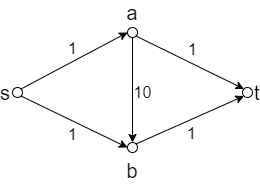
\includegraphics[scale=0.5]{image/network-flow-greedy-example.png}
		\caption{一个网络流算例}
	\end{figure}\label{fig:max-flow-greedy-fig1}
	\par 容易看出这个例子的最大流为2,即通过\(s \to a \to t\)和\(s \to b \to t\)两条路径各输送1个流量。
	但上述贪心算法不能保证这个结果,因为它第一次找到的路径可能是\(s \to a \to b \to t\),则输送流量后,
	剩余容量更新为以下形式。

	\begin{figure}[hbt]
		\centering
		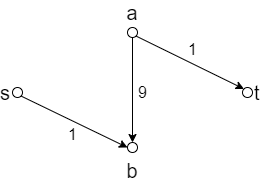
\includegraphics[scale=0.5]{image/network-flow-greedy-example2.png}
		\caption{通过路径\(s \to a \to b \to t\)输送1个流量后的容量剩余情况}\label{fig:max-flow-greedy-fig2}
	\end{figure}
	\par 此时,图中不再有\(s \to t\)的路径,贪心算法结束,但求得的结果不是最大流。

\end{example}

	\par 尝试更换另一种贪心策略,如最短路径优先,可不可行呢?
	只需将\autoref{fig:max-flow-greedy-fig1}中的图修改为以下形式,
	在\autoref{fig:max-flow-greedy-fig3}中,\(s\)到\(b\)和\(a\)到\(t\)之间各有十个以上的点依次相连,各边容量都大于等于1,
	易知最大流的值也是2。
	但此时,贪心算法仍会选择路径\(s \to a \to b \to t\),因为它最短,从而得到同样的错误结果。

	\begin{figure}[hbt]
		\centering
		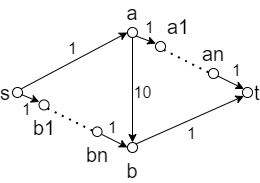
\includegraphics[scale=0.5]{image/network-flow-greedy-example3.png}
		\caption{最短路径优先的贪心策略的反例}\label{fig:max-flow-greedy-fig3}
	\end{figure}

	\par 简单的贪心策略似乎不能有效求解最大流问题,那么正确的方法是什么呢?

\subsection{Ford-Fulkerson算法}

	\par Ford-Fulkerson算法于1956年提出,简称FF算法,直到现在仍是许多现代最大流求解算法的基础。
	严格地说,FF算法并不是“算法”,而是一种方法,因为其中的一些操作是不确定的,需要实现者自行选择策略。
	
	\par FF算法的主要思想是允许反悔。也就是说,当流量经过了一条不合适的路径后,能够反悔,进行回溯。
	如何实现这一机制呢?如何保证反悔后不会重蹈覆辙?首先引入残差图的概念。

\begin{definition}{残差图}{residual-graph}
	残差图也是一个有向图。对给定的图\(G(V,E)\)和图上现有的一个流\(f\),构造对应的残差图,记为\(G_f\)。
	构造规则如下:
	\begin{enumerate}[(1)]
		\item 对\(G\)中的所有有流量的边\(e=(u,v),\ u,v\in V\),在残差图\(G_f\)中加入该边,
			其残差容量\(C_f(e)=C(e)-f(e)\)。
			同时,也向\(G_f\)中加入其反向边\(e'=(v,u)\),其中\(C_f(e')=f(e)\);
		\item 在残差图\(G_f\)上操作流量时,所有边都是可走的。在路径上输送流量时,同样更新路径上所有边的残差容量\(C_f\)。
			若对某一个边\(e\),它没有反向边,则按同样规则加入反向边,若已有反向边\(e'\),则使\(C_f(e')\)增加新流量的值;
		\item 当\(G_f\)中某一边的的残差容量减至0时,将其从\(G_f\)中去掉。
	\end{enumerate}
\end{definition}

	\par 由残差图的构造方式可知,当\(G\)中没有流量时,\(G_f\)与\(G\)是相同的。对\autoref{fig:max-flow-greedy-fig2}中的情况,
		给出对应的残差图,如\autoref{fig:residual-graph1}所示。当在路径\(s \to a \to b \to t\)上输送一个流量后,
		\((s,a),\ (b,t)\)上的残差容量减为0,从残差图中去掉;\((a,b)\)上的残差容量减少1;同时为路径上的所有边更新了反向边。
	
		\begin{figure}[hbt]
			\centering
			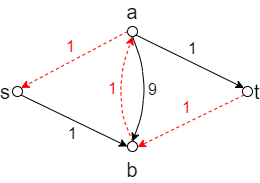
\includegraphics[scale=0.5]{image/network-flow-residual-graph1.png}
			\caption{通过路径\(s \to a \to b \to t\)输送1个流量后的残差图}\label{fig:residual-graph1}
		\end{figure}


	\par 在残差图的基础上,引入增广路径的概念。

\begin{definition}{增广路径}{argument-path}
	对给定的图\(G(V,E)\)和图上现有的一个流\(f\),一条增广路径是相应的残差图\(G_f\)上的一条从\(s\)到\(t\)的简单路径。
\end{definition}

	\par 引入残差图和增广路径的概念,通过添加反向边,提供了一种反悔回溯的方式,这就是FF算法的妙处。以下给出FF算法的描述。

\begin{algorithm}[hbt]
	\caption{Ford-Fulkerson算法}\label{alg:ford-fulkerson}
	\KwIn{图$G$}
	\KwData{流的值$f$ = 0}
	\Begin{
		由$G$得到残差图$G_f$\\
		\While{$G_f$中存在增广路径}{
			选择某一条增广路径输送流量,并更新路径上各边和反向边的残差容量\\
			$f$增加输送流量的大小
		}
	}
	\Return{$f$}
\end{algorithm}

	\par 对于\autoref{fig:residual-graph1}中的情形,FF算法还可在图中找到\(s \to b \to a \to t\)这样一条增广路径,
	相当于对先前走边\((a,b)\)进行了反悔,最终找到了最大流。

	\par 从FF算法的描述中可以注意到,其中确实存在不明确的操作,也就是未提及增广路径的选择策略。
	不同的选择策略可能会带来性能上差异,这里暂时不讨论。

	\par 有了FF算法,如何说明其正确性呢?通过以下引理,可以证明FF算法是正确的。

\begin{lemma}{}{max-flow-lemma1}
	对于给定的图\(G(V,E)\)和一个流\(f\),以下命题是等价的:
	\begin{enumerate}[(1)]
		\item \(f\)是最大流;
		\item \(G\)的残差图\(G_f\)中,不存在\(s \to t\)的路径,即增广路径。
	\end{enumerate}
\end{lemma}

\begin{proof}
	\begin{enumerate}[a)]
		\item (1) $\rightarrow$ (2):

			采用反证法,即证明$\neg$ (2) $\rightarrow$ $\neg$(1)。
			假设\(f\)是最大流,若\(G_f\)中仍存在增广路径,设其瓶颈容量为\(\Delta f\),
			则从\(s \to t\)还可以输送\(\Delta f\)的流量,即存在大小为\(f + \Delta f\)的流,使得
			\begin{equation}\nonumber
				f + \Delta f > f
			\end{equation}
			因此\(f\)不是最大流。
		\item (2) $\rightarrow$ (1):

			在残差图\(G_f\)中,将从源点\(s\)出发仍有路径可达的所有点以及源点\(s\)设为点集\(A\),图中的其他点构成点集\(B\)。
			因为\(G_f\)中不存在\(s \to t\)的路径,所以\(t \in B\),由定义\ref{def:s-t-cut}可知,这实际上构成了一个\(s-t\)割\(cut(A,B)\)。
			\begin{figure}[hbt]
				\centering
				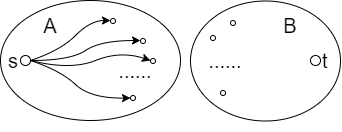
\includegraphics[scale=0.5]{image/network-flow-ff-proof-graph1.png}
				\caption{构造一个\(s-t\)割}\label{fig:ff-proof-graph1}
			\end{figure}

			在原图\(G\)中,由连通性的要求,一定存在点集\(A\)与点集\(B\)之间的边,这些边中有从\(A\)到\(B\)的,也可能有从\(B\)到\(A\)的,
			如\autoref{fig:ff-proof-graph2}所示。
			
			对于从\(A\)到\(B\)的边,如\((a_1,b_1)\),边上的流量\(f(a_1,b_1)\)一定是等于边的容量\(C(a_1,b_1)\)的,
			否则,在残差图\(G_f\)中,\((a_1,b_1)\)的残差容量\(C_f(a_1,b_1)\)就不为0,使得仍有从\(A\)到\(B\)的路径。
			
			对于从\(B\)到\(A\)的边,如\((b_n,a_3)\),边上的流量\(f(b_n,a_3)\)一定为0,
			否则,在残差图\(G_f\)中就会存在反向边\((a_3,b_n)\),且其残差容量为\(f(b_n,a_3)\)的值,也使得从\(A\)到\(B\)有路径。
			\begin{figure}[hbt]
				\centering
				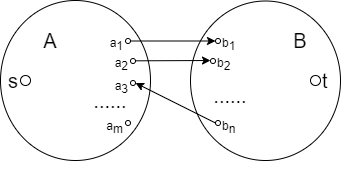
\includegraphics[scale=0.5]{image/network-flow-ff-proof-graph2.png}
				\caption{原图\(G\)上的\(cut(A,B)\)}\label{fig:ff-proof-graph2}
			\end{figure}

			基于上述观察,对于\(cut(A,B)\),有
			\begin{equation}\nonumber
				\begin{split}
				|f| = f(A, B)& = \sum_{u \in A, v \in B, (u,v) \in E} f(u,v) - \sum_{u \in A, v \in B, (v,u) \in E} f(v,u)\\
				& = \sum_{u \in A, v \in B, (u,v) \in E} f(u,v)\\
				& = C(A, B)
				\end{split}
			\end{equation}

			因为流\(f\)是不依赖于\(s-t\)割的,根据性质\ref{pro:s-t-cut-capacity-prop},对于一个图上任意的\(s-t\)割,流值总是小于其容量的,
			也就是说,任何流的值总小于等于容量最小的\(s-t\)割的容量。
			此时,流\(f\)的值等于\(C(A,B)\),表明\(cut(A,B)\)就是容量最小的\(s-t\)割,而\(f\)就是最大流。

	\end{enumerate}
\end{proof}

	\par 在FF算法中,算法会运行至残差图中没有增广路径为止,结束时求得的流就是最大流。以上证明也间接证明了其正确性。
	此外,由该证明过程可以导出一个定理,即最大流最小割定理。

\begin{theorem}{最大流最小割定理}{maximum-flow-minimum-cut-theorem}
	对于一个有向图\(G\),其最大流的值等于其容量最小的\(s-t\)割的容量值。
\end{theorem}

\subsection{Ford-Fulkerson算法的实现及其时间复杂度}
\par 基于DFS实现的FF算法是FF算法的最基础的实现形式,其算法描述如下

\begin{algorithm}
\caption{基于DFS的FF算法}\label{alg:ford-fulkerson}
\KwIn{图 $G$,其中$s$和$t$分别为其源点和汇点}
\KwData{流的值$f$ = 0}
\Begin{
	$tmp$ = dfs($G$, $s$, $inf$)

	\While{$tmp$ > 0}{
		$f$ = $f$ + $tmp$
	}
	\Return{$f$}
}

\end{algorithm}

\par 其中,dfs()算法通过深度优先的方式在图$G$中寻找增广路径,并返回所找到的增广路径的流量。同时,按照FF算法的要求,其在寻找增广路径的过程中会更新增广路径上各边的残差容量。其实现可以描述如下

\begin{algorithm}
\caption{dfs()}
\KwIn{图$G$,当前节点$p$,当前流值$flow$}
\KwData{流值$ret$}
\Begin{
	\If{$p$ = $t$} {
		\Return{$flow$}
	}
	\For{$next$为$p$的下一节点}{
		$tmp$ = dfs($G$,$p$,min($flow$,c($p$,$next$)))

		\If{$tmp$ > 0}{
			c($p$,$next$) = c($p$,$next$) - $tmp$	
	
			c($next$,$p$) = c($next$,$p$) + $tmp$

			\Return{$tmp$}
		}
	}
	\Return{0}
}
\end{algorithm}

\par 不难推算出,该算法的时间复杂度为$O(mf)$,其中$m$为图$G$中边的数量,$f$为最大流。同时,需要注意的是,该算法并不能有效的处理环的情况。当图中存在环的时候,该算法很有可能陷入无限的循环之中。当然,这可以通过众多的改进措施避免。

\par 然而,现在最常见的网络流算法是Dinic算法。其可以有效的避免因为图中存在环状结构而陷入死循环的问题。同时,因为采用了分层的机制,其时间复杂度也有所降低,为$O(m^2n)$。给出Dinic算法的伪代码描述如下。

\begin{algorithm}
\caption{Dinic()}
\KwIn{图$G$}
\KwData{最大流值$f$}
\Begin{
	$f$ = 0

	\While{bfs($G$) != 0}{
		$tmp$ = dfs($G$,$s$,$inf$)

		\If{$tmp$ <= 0} {
			\Return{$f$}
		}
		$f$ = $f$ + $tmp$
	}
}
\end{algorithm}

\par 其中,bfs()算法负责为当前的图按照广度优先的策略“分层”,并返回$t$点的层数。分层的主要目的是加速dfs()算法查找增广路径的速度,并避免算法陷入死循环之中。dfs()算法则与上文中提到的类似,但其每次迭代均只会选择层数高于当前节点的节点。下文给出bfs()算法的代码描述。而dfs()算法则可在上文dfs()算法的基础上进行简单修改得到。

\begin{algorithm}
\caption{bfs()}
\KwIn{图$G$,其中所有节点的层数均为0}
\KwData{节点$t$的层数}

\Begin{
	将$s$的层数设置为$level$

	将$s$压入栈$stack$中

	\While{$stack$不为空}{
		从$stack$中出栈节点$node$,其层数为$level$

		\For{$n$为$node$的子节点}{
			\If{$n$的层数为0}{
				将$n$的层数设置为$level$+1

				将$n$压入$stack$
			}
		}
	}

	\Return{$t$的层数}
}
\end{algorithm}

\par 当然,除了上述的两种FF算法的实现外,还有众多算法可以实现FF算法所描述的思想。诸如WAP(Widest Argumentary Path)算法、SAP(Shortest Argumentary Path)算法等。这些算法着眼于优化FF算法中寻找增广路径的部分,并且较之基本的FF算法有着更优的时间复杂度。限于篇幅此处不一一赘述,感兴趣的读者可以自行去查找相关资料。

\subsection{FF算法的局限性}

\par 我们可以看到,FF算法能够很好地解决边权为有理数的图的最大流问题,但其无法很好地解决边权为无理数的图的最大流问题。我们可以通过一个例子来解释这个问题。假设有$r^2=1-r$,考虑下图的情况

\begin{figure}[hbt]
	\centering
	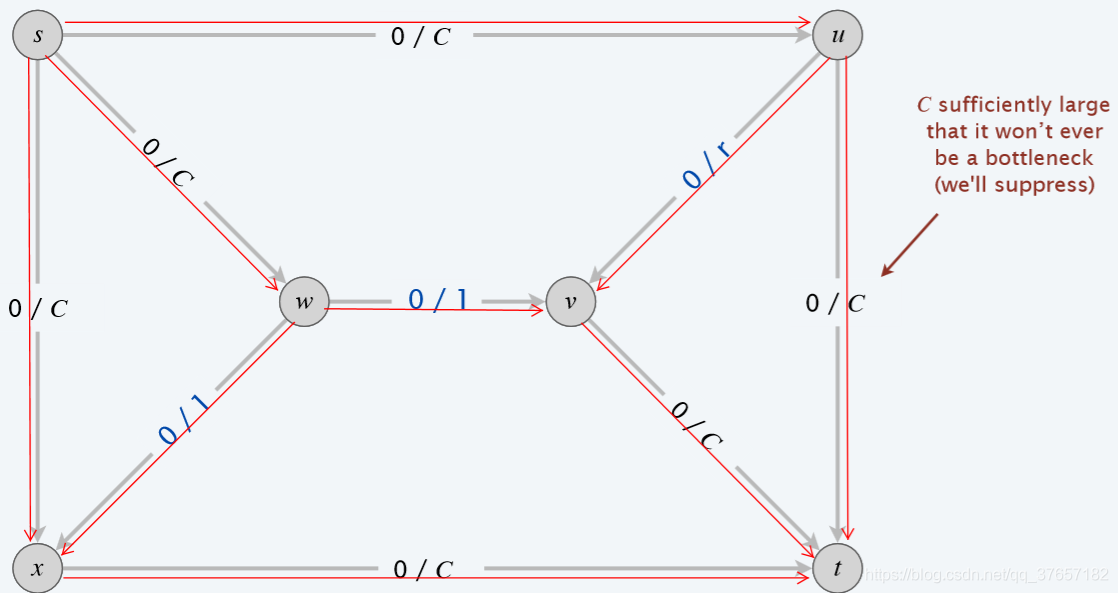
\includegraphics[scale=0.4]{image/network-flow-backbone1.png}
	\caption{Ford-Fulkerson算法的缺陷(1)}\label{fig:network-flow-backbone1}
\end{figure}

\begin{figure}[hbt]
	\centering
	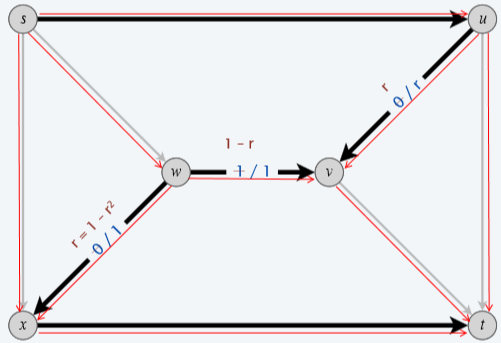
\includegraphics[scale=0.6]{image/network-flow-backbone2.png}
	\caption{Ford-Fulkerson算法的缺陷(2)}\label{fig:network-flow-backbone2}
\end{figure}

\begin{figure}[hbt]
	\centering
	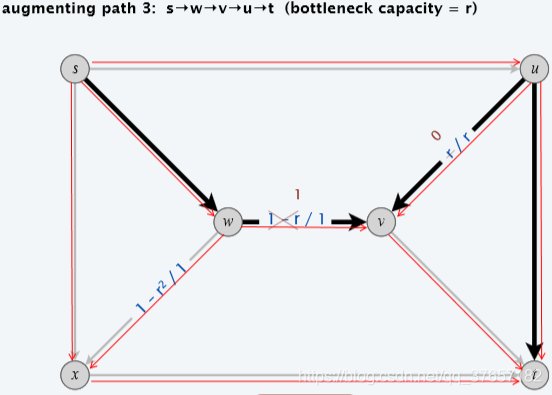
\includegraphics[scale=0.6]{image/network-flow-backbone3.png}
	\caption{Ford-Fulkerson算法的缺陷(3)}\label{fig:network-flow-backbone3}
\end{figure}

\begin{figure}[hbt]
	\centering
	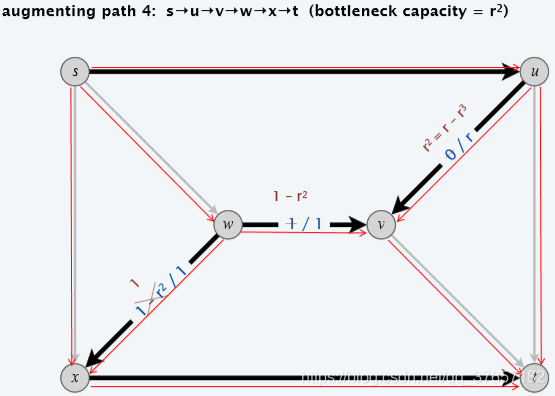
\includegraphics[scale=0.6]{image/network-flow-backbone4.png}
	\caption{Ford-Fulkerson算法的缺陷(4)}\label{fig:network-flow-backbone4}
\end{figure}

\begin{figure}[hbt]
	\centering
	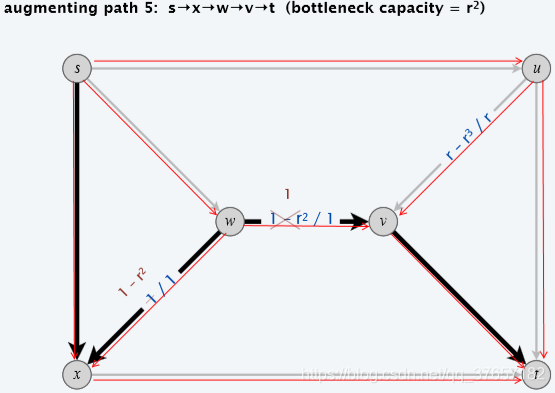
\includegraphics[scale=0.6]{image/network-flow-backbone5.png}
	\caption{Ford-Fulkerson算法的缺陷(5)}\label{fig:network-flow-backbone5}
\end{figure}

\begin{figure}[hbt]
	\centering
	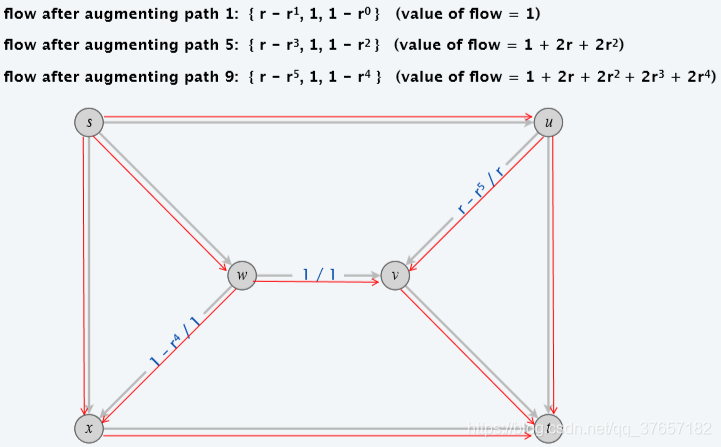
\includegraphics[scale=0.6]{image/network-flow-backbone6.png}
	\caption{Ford-Fulkerson算法的缺陷(6)}\label{fig:network-flow-backbone6}
\end{figure}

\par 可以看见,FF算法并不会停下来。相反的,因为各边边权的这种奇妙的关系,算法会无休止地运行下去。其所得到的流值最终仍会收敛,但却会收敛到一个错误的值上。从这个例子可以看到,FF并不适合于某些边权为无理数的图。
\input{src/Network-flows.tex}
\chapter{网络流应用之图像分割}

\centering{本章简单介绍网络流在图像分割上的应用。}
{\centering 本章简单介绍网络流在图像分割上的应用。}

\begin{definition}{背景知识}{}
	图像是可以看作由一个个像素组成的巨大图, 将像素一一用边连接起来, 则这些像素点会成为这个巨大图网络的顶点.
	一个图由前景和背景组成, 假设顶点上的值用 $a_i$ 表示, $ 0 \leq a_i \leq 1 $,  $a_i$ 趋近于 0 表示 $a_i$ 为图的背景, $a_i$ 趋近于 1 表示 $a_i$ 为图的前景, 并且设所有属于前景的顶点 $a_i$ 构成集合 A, 所有属于背景的顶点 $a_j$ 构成集合 B.
	假设边上的值用 $w_{ij}$ 表示, $w_{ij}$ 设为边的惩罚值, $w_{ij}$ 趋向于 0 表示“分离” (即 $w_{ij}$ 连接的两个点分别属于前景和背景), $w_{ij}$ 趋向于 1 表示“在一起” (即 $w_{ij}$ 连接的两个点都属于前景或者背景)
	设总的惩罚值为 $ A = \min\left(\sum_{i \epsilon B}a_i +  \sum_{i \epsilon A}(1 - a_j) + \sum_{i \epsilon A, j \epsilon B}w_{ij} \right) $
\end{definition}


\section{问题实例}
\subsection{问题描述}
\begin{itemize}
	\item 对于下面这个图,利用网络流求解该图前景和背景的最大可能
\end{itemize}

\begin{figure}[htb]
	\centering
	\includegraphics[scale=0.8]{image/Image-segmentation2.png}
	\caption{图片前景背景识别}\label{fig:image-seg-1}
\end{figure}

\subsection{思路描述}
\begin{itemize}
	\item 图形切割算法通过向图 G (V,E) 添加 S 点和 T 点,将图中所有的顶点,与 S 和 T 建立边,
	      如果一个点与 S 相连,则对应边的权值为该点的值 $a_i$, 如果一个点与 T 相连,则对应边的权值为1减去该点的值 $ 1 - a_j $。
	      可以得到下面这个图:
\end{itemize}

\begin{figure}[htb]
	\centering
	\includegraphics[height=4.5cm]{image/Image-segmentation3.png}
	\caption{图片前景背景识别}\label{fig:image-seg-2}
\end{figure}

\begin{itemize}
	\item   根据最大流最小割, 可以得到得到二分图的最大匹配, 可以得到集合A和B, 保证总的惩罚值 $ A = \min\left(\sum_{i \epsilon B}a_i +  \sum_{i \epsilon A}(1 - a_j) + \sum_{i \epsilon A, j \epsilon B}w_{ij} \right) $ 最小,
	      最小为 $(0.2 + 0.1) + (1 - 0.9) + (1 - 0.8) + 0.3 + 0.3 = 1.2 $, 而 A 和 B 分别对应图的前景和背景。
\end{itemize}

\section{问题扩展}
\begin{itemize}
	\item 假如一个图的前景不是一个整体,
	      而是有两个分开的部分,比如两只在两个不同位置的猫在一个图中。
	      这样一个算法能否将图像上的前景和背景分开?
\end{itemize}

\begin{figure}[htb]
	\centering
	\includegraphics[scale=0.6]{image/Image-segmentation1.png}
	\caption{图片前景背景识别}\label{fig:image-seg-3}
\end{figure}

	
	\chapter{P/NP 基本概念}
	
	\begin{introduction}
		\item $P$,$NP$,$NPC$,$NP-Hard$问题定义
		\item 多项式时间归约
		\item NPC问题概述
		\item P与NP的讨论
	\end{introduction}
	
	\section{引入}
	\begin{table}[!htbp]
		\centering
		\caption{不同算法的复杂度}
		\begin{tabular}{cc}
			\toprule[0.5mm]
			Easy Problem & Hard Problem\\
			(存在多项式复杂度的确定性算法)&(不知道是否存在多项式复杂度的确定性算法)\\
			\midrule[0.4mm]
			最短路问题&最长路径问题\\ \\
			2SAT问题&3SAT问题\\ \\
			2色问题&3色问题\\ 
			\bottomrule
		\end{tabular}
	\end{table}
	
	\section{概念辨析}
	\begin{definition}{$P$类问题}{def1}
	$P$代表\textit{Polynomial},指存在多项式复杂度的算法的问题。
	\end{definition}

	\begin{definition}{$NP$类问题}{def1}
	$NP$代表\textit{Non-deterministic Polynomial},指可以在多项式时间内验证一个解,或有一个多项式时间的非确定性算法的问题。
	\end{definition}

	\begin{definition}{$NPC$类问题}{def3}
	$NPC$代表\textit{Non-deterministic Polynomial Complete},指满足以下两个条件的问题:
	
	(1)它是一个$NP$问题。
	
	(2)所有的$NP$问题都可以在多项式时间归约到它。
	\end{definition}

	\begin{definition}{$NP-Hard$类问题}{def4}
		指满足$NPC$问题的第二条,但不一定要满足第一条的问题。
	\end{definition}
	
	为了更好的阐述这种关系,我们采用它们之间的关系图来对此进行描述,见\autoref{fig:relation-of-three-questions}:
	
	\begin{figure}[ht]
		\begin{minipage}[t]{1\linewidth}
			\centering
			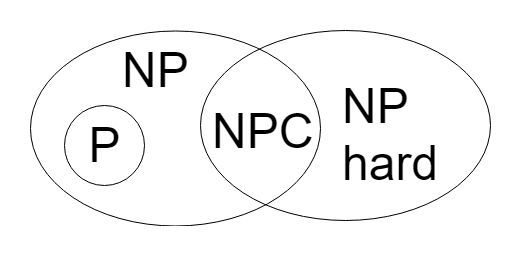
\includegraphics[width=10cm,height=5cm]{image/P_NP1.png}
			\caption{$P$,$NP$,$NPC$,$NPhard$关系图}\label{fig:relation-of-three-questions}
		\end{minipage}
	\end{figure}
	
	\section{多项式时间归约}
	\subsection{多项式时间归约的定义与性质}
	在讨论$NPC$问题时我们谈到了多项式时间规约,这里给出了多项式时间规约的定义:
	\begin{definition}{多项式时间规约}{def5}
	多项式时间归约:如果问题$X$和问题$Y$满足以下两条性质,那么问题$X$可以在多项式时间归约到问题$Y$,记作$X\leq_pY$:
		
	(1)问题$X$可以通过多项式时间的基本运算步骤转换为问题。
	
	(2)问题$X$多项式次调用求解问题Y的算法。
	\end{definition}
	有关多项式时间规约,有以下四条性质:
	\begin{theorem}{多项式规约的四条性质}{}	
		\begin{enumerate}
			\item 如果$X\leq_pY$且$Y$能在多项式时间内求解,则$X$也能在多项式时间内求解。
			\item 如果 $X\leq_pY$,且$Y$不能在多项式时间内求解,则$X$也不能在多项式内求解。
			\item 如果$X\leq_pY$且$Y\leq_pX$,则$X$,$Y$多项式等价,记为$X\equiv_pY$。若$X$,$Y$中一方能在多项式时间内求解则另一方也能在多项式时间内求解。
			\item 归约的传递性:若$Z\leq_pY$且$Y\leq_pX$,则$Z\leq_pX$。
		\end{enumerate}
		
	\end{theorem}

\paragraph*{以下有三点提醒:}

\begin{itemize}
	\item 注意体会上述两个定理中$X$与$Y$的表达顺序;
	\item 第二条定理的证明可以采用反证法,假设$X$可以在多项式时间内求解,因为$Y$能够在多项式时间内归约到$X$问题求解,所以$Y$也能在多项式时间内求解,矛盾;
	\item $X$的问题比$Y$更“难”。
\end{itemize}

	\subsection{规约问题的举例——染色问题(Graph Coloring)}

\begin{itemize}
\item $P_1$ (decision version):可用$K$种颜色完成染色
\item $P_2$ (optimal version):最少用$K$种颜色完成染色
\end{itemize}

以下有两种情况:


	\begin{enumerate}
	\item $P_1\leq_pP_2$
	
将$K$值依次从2依次递增,直到$P_1$判定第一个满足的数记为$K_0$,则$K_0$为$P_2$的解,即满足$P_1$的最小的$K$(也就是$K_0$)为$P_2$的解。

过程见\autoref{fig:P1-leq-P2}:


	\begin{figure}[ht]
		\begin{minipage}[t]{1\linewidth}
			\centering
			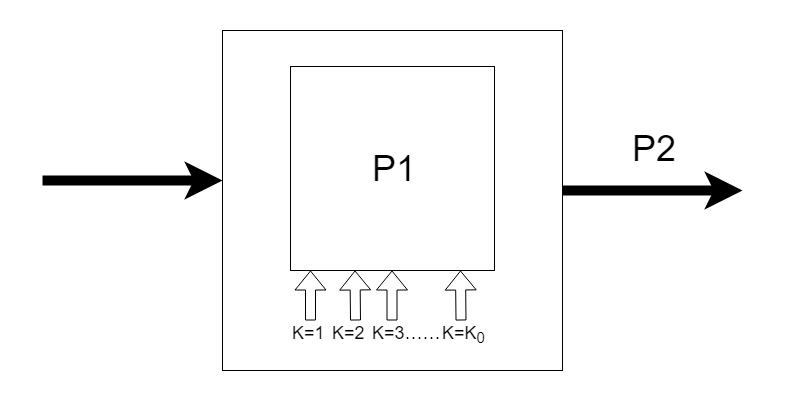
\includegraphics[width=15cm,height=7.5cm]{image/P_NP2.png}
			\caption{$P_1\leq_pP_2$时过程图}\label{fig:P1-leq-P2}
		\end{minipage}
	\end{figure}


	\item  $P_2\leq_pP_1$
	
	直接利用$P_2$解出$K_0$,判断$K$与$K_0$的关系,若$K\geq K_0$则成立,即可以使用$K_0$种颜色完成染色。
	
过程见\autoref{fig:P2-leq-P1}:
	\end{enumerate}
	

		\begin{figure}[ht]
		\begin{minipage}[t]{1\linewidth}
			\centering
			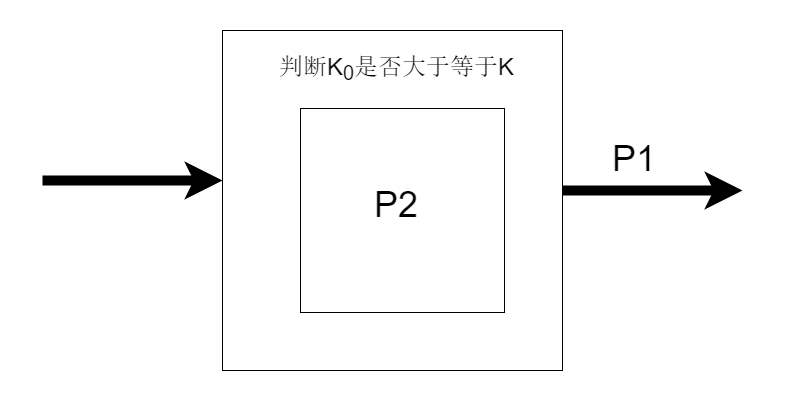
\includegraphics[width=15cm,height=7.5cm]{image/P_NP3.png}
			\caption{$P_2\leq_pP_1$时过程图}\label{fig:P2-leq-P1}
		\end{minipage}
	\end{figure}
	
\newpage
	\section{NPC问题}
	\subsection{NPC概述}

\paragraph*{$NPC$问题的证明思路}

	
要证明一个问题是$NPC$问题,先证明它是一个$NP$问题,然后再证明一个已知的$NPC$问题能在多项式时间归约到它。

\paragraph*{$NPC$问题与$NP$问题之间的关系}


$NPC$问题是比普通的$NP$问题更复杂一点的问题,如果找到一个$NPC$的多项式复杂度算法,也就能够通过降阶的方式将这个算法改造成解决任意一个确定的$NP$问题的多项式复杂度算法。意味着存在一个通用的万能算法,能够解决所有$NP$问题,这样只要找到一个$NPC$的多项式算法也就证明了$P=NP$。
	
\paragraph*{$NPC$问题举例}
	\subparagraph*{}
	
	\begin{table}[ht]
		\centering
		\caption{NPC问题举例}
		\begin{tabular}{p{100pt}p{200pt}}
			\toprule[0.5mm]
			问题 & 描述\\
			\midrule[0.4mm]
			布尔可满足性问题&给定一个布尔方程,判断是否存在一组布尔变量的真值指派使整个方程为真的问题\\ \\
			最小顶点覆盖问题&给定图$G=(V,E)$和数$k$,判定是否存在包含大小至多为$k$的顶点覆盖。\\ \\
			集合覆盖问题&给定全集$U$,以及一个包含$n$个集合且这$n$集合的并集为全集的集合$S$。集合覆盖问题要找到的一个最小的子集$S$,使得他们的并集等于全集\\ \\
			哈密尔顿回路&给定图$G$,判定其是否经过图中每个顶点且仅一次的回路。\\
			\bottomrule
		\end{tabular}
	\end{table}
\section{关于P与NP的讨论 (P=NP?)}

\begin{itemize}
	\item$P\subseteq NP$

如果一个问题能够在多项式时间求解,那么这个问题则一定可以在多项式时间内被验证

	\item $P$是否能够等于$NP$,即等价于一个问题的结果如果能够用多项式复杂度的算法来验证,那么是否存在多项式算法来得出这个结果。现在没人能够证明这一点。
	\item 证明的关键点在于能否找到一个$NPC$的多项式算法。但$NPC$问题目前没有多项式算法,只能用穷举法逐个检验得到答案。所以现在科学家们普遍认为$P\neq NP$
	\item 假设证明了$P= NP$,目前的加密技术就会没有前途,因为目前的加密技术是将一个整数分解为几个因数的乘积,正是因数分解过程烦琐,才保证了信息的安全。
\end{itemize}
	
以下列出了$P= NP$与$P\neq NP$两种情况的情况见\autoref{fig:P-eq-NP}和\autoref{fig:P-neq-NP}:
	
	\begin{figure}[!htbp]
		\begin{minipage}[t]{1\linewidth}
			\centering
			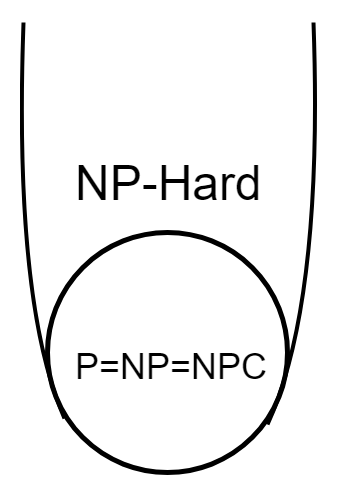
\includegraphics[width=4cm,height=6cm]{image/P_NP4.png}
			\caption{$P= NP$时关系图图}\label{fig:P-eq-NP}
		\end{minipage}
	\end{figure}

		\begin{figure}[!htbp]
		\begin{minipage}[t]{1\linewidth}
			\centering
			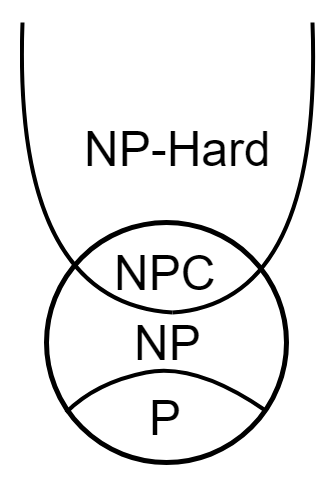
\includegraphics[width=4cm,height=6cm]{image/P_NP5.png}
			\caption{$P\neq NP$时关系图} \label{fig:P-neq-NP}
		\end{minipage}
	\end{figure}
	


\bibliography{ref.bib}
\end{document}
